\hl{L9: ScalableGNN}
Train a GNN in large-scale graph is hard: load the entire graph and features, (1)requiring memory becomes prohibitively large, (2)inefficient gradient update due to minibatch sampling.
\textbf{Three techs:1)Data level: graph sampling, 2)Model level: simplifying GNNs, 3)System level: distributed learning} \hlorange{Graph Sampling}: Cannot sample directly sample nodes because 
it's Necessary to preserve structure information.     \textbf{\textcolor{red}{Node-wise sampling}}: \textbf{Mini-batch training}: Randomly sample a few nodes, leverage computational graph (a node and its neighbor, neighbor's neighbr ...) to aggregate k-hop neighbors, obtaining their embedding and training. \textbf{problem}:neighbor explosion when 1)layer size grows 2)meet high degree nodes. \textbf{GraphSage}:sample neighbors in computational graph. \underline{How to sample?}1) random sample: fast but may sample unimportant nodes. 2) Random Walk with Restarts (
\textcolor{red}{RWR}):Use RWR score to measure the node importance. \underline{Time complexity}: $M*m^K$, M is number of sampled nodes, m is the maximum sampled neighbor number, K is the number of layers. \underline{Limitations}:1) neighbor explosion when m and K are large 2)Smaller m leads to unstable training due to the larger variance in neighbor aggregation. 3)Computation is redundant when nodes in a mini-batch share many neighbors \textbf{GNNAutoScale}: steps: 1)select a mini-batch of nodes,2)only sample one hop (full) neighbors for each node in message passing. (to tackle the issue: GNN may lose out-of-mini-batch information,3)use historical embeddings to approximate the missing out-of-mini-batch information. \underline{Pros}:a)avoid neighborhood
explosion issue, b)low variance c)Reduce redundant computations \underline{Cons}:a)The approximation error leads to performance drop, b) Historical embeddings require CPU memory storage. \textbf{\textcolor{red}{Subgraph-wise Sampling}}: sample small graphs. Motivation: Real-world graph exhibits community structure. Each community retains essential local connectivity patterns of the original graph. \hlorange{Vanilla Cluster-GCN}: First, Use any community detection algorithms (Louvain, METIS) to partition nodes into clusters. Then, for each mini-batch, randomly sample a node group and construct the induced graph. Any GNN message passing over the induced subgraph to compute the loss. \underline{Cons}: 1) Message passing is not available between clusters, which could hurt the performance 2) Unreliable gradients: Community detection algorithm tends to bring similar
nodes together. Unbalanced data distribution of a subgraph causes biased gradient estimation and slow convergence of SGD. \hlorange{Advanced Cluster-GCN}: partition small groups of nodes, for each mini-batch, sample and aggregate multiple node groups, then construct the induced subgraph.\underline{Complexity}: The subgraph contains $M*D_{avg}$ edges, where $D_{avg}$ is the average node degree. K-layer message passing over the subgraph costs at most $K*M*D_{avg}$, linear dependency w.r.t. $K$. \hlorange{Simplified GCN}: Key-idea: simplify GCN by removing the non-linear activation (r.g. ReLU) from the GCN. 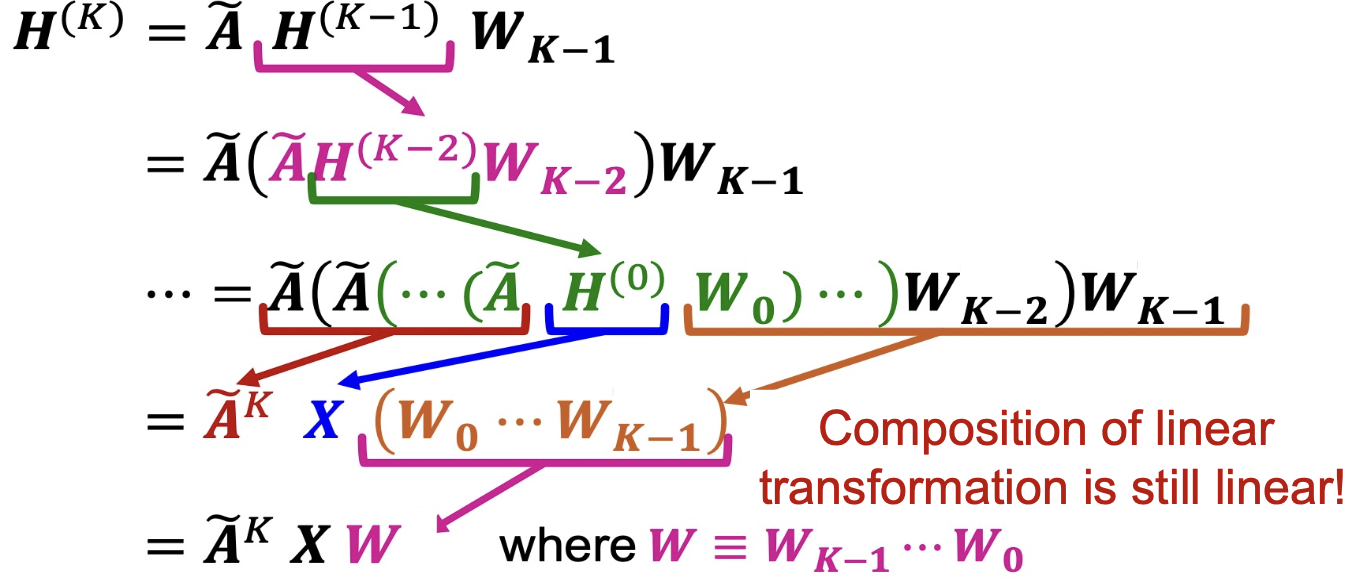
\includegraphics[height=0.06\textwidth]{figs/l9-1.png}  Notice that $\widetilde{X} = \widetilde{A}^KX$ contains no trainable parameter, so it can be pre-computed. Finally, implified GCN’s embedding is $H^{(K)} = \widetilde{X}W$, it’s just a linear transformation of precomputed matrix. For node $v$,its final embedding $h^k_v$ is $h^k_v=\widetilde{X}_vW$. \underline{Limitations}: Compared to the original GNN models, simplified GCN is less expressive as it removes the non-linearity. When does simplified GCN work? 1)Simplified GCN generates similar pre-processed features
for neighboring nodes. 2)Work well on homophilous graphs (neighboring nodes tend to share the same target labels). \hlorange{Distributed Learning}: Def: two or more machines collaborate on a single machine learning task. Require explicit (i.e. written in software) communication among the machines. \underline{Basic concepts}:\textbf{Push}: machine A sends some data to machine B. \textbf{Pull}: machine B requests some data from machine A. \textbf{All-Reduce}: compute some reduction (e.g., a sum) of data on multiple machines and synchronize the result on all those machines. \textbf{Data parallelism}: different machines have a complete copy of the model and a part of the data.\textbf{Model parallelism}: different machines are responsible for computation in different parts of a single model. \underline{Graph Partition} The input graph along with the features is partitioned across multiple machines. Partition schemes: random, edge-cut partitioner, or vertex-cut partitioner. \underline{Computation Graph Generation}Create the computation graph of each node in the mini- batch by pulling its k-hop neighborhood and the associated features. Require communication with other machines. \underline{Data Parallelism} Parallelize the mini-batch data on multiple machines and synchronize the gradients. \underline{Issue: Communication Bottleneck}: K-layer GNNs need to pull and aggregate the features of K- hop neighbors of nodes in each mini-batch training. Communication overhead dominates training time (GPUs are being underutilized).\underline{$P^3$} $P^3$ proposes push-pull parallelism for distributed GNNs that effectively eliminates the communication overhead. Key insights:1)The transmission of features causes dominant network traffic → avoiding feature movements.2)Existing system consider graph and features indivisible → independent partitioning of structure and features. \underline{$P^3$: Independent Partitioning}: Graph structure: partitioned using random scheme. pNode features: partitioned along feature dimension.\underline{$P^3$: Computation Graph Generation}Each machine samples a batch of nodes, then pulls the computational graph of each node. Features are not pulled, which reduces the network overhead of feature movement. Then, each machine pushes the locally created computational graphs to all other machines. \underline{$P^3$: Hybrid Parallelism} Model parallelism: each machine computes partial hidden node embeddings using the partial input features it owns. Each machine pulls the partial embeddings of nodes from other machines and aggregate them using reduce operation. GNNs typically use small hidden dimensions. The transmission of hidden embeddings incurs much less overhead compared to transferring original features. \underline{$P^3$: GNN training} Hybrid parallelism requires communication in forward and backward pass, which needs to pull partial hidden embeddings in the forward pass and push the gradients in the backward pass. \underline{$P^3$: Limitation}: It basically assumes the hidden dimension in GNNs is small. The benefits of $P^3$ decreases when increasing the number of hidden dimensions.


\hl{L10: AutoML on Graphs}
\hlgreen{AutoML}: Automated Machine Learning (AutoML) is the process of automating the tasks of applying machine learning to real-world problems. Neural Architecture Search (NAS) is a technique for automating the design of artificial neural networks. \hlgreen{AutoML on Graphs}: Two main directions: 1)Graph Neural Architecture Search (NAS), aimis to find the GNN architecture that can achieve the optimal performance on a given graph data 2) Hyper Parameter Optimization (HPO), aims to automatically find the optimal hyper-parameters of the GNN Model. \hlorange{Advantages of AutoML}: 1) Free humans out of the loop. 2) High optimization efficiency. 3)Discover and extract patterns and combinations automatically. \hlgreen{search space}: The search space in AutoGNN is differentiated according to GNN architectures and training hyperparameters. \underline{1)Micro-architecture:} To represent a graph convolutional layer,including \hlblue{hidden units} (feature dimensions, like 4,16,128), \hlblue{propagation} function (the function to compute the weight between nodes, like adjacency, GAT ...), \hlblue{aggregation func} (like SUM, MEAN, MAX), \hlblue{Combination func} (The function used to combine the embeddings of neighbors and node itselfs, like MLP), \hlblue{activation func} (ReLU, Sigmoid, Tanh, softmax...)\underline{2)Macro-architecture}: To represent network topology, including the \hlblue{layer depth}, \hlblue{inter-layer skip connections} e.g. [SUM, CAT, MAX, LSTM], and \hlblue{pre/post processing layers}. \underline{3) Hyperparameter}:\hlblue{drop out rate}, \hlblue{learning rate}, \hlblue{batchnorm} e.g. [False, BatchNorm, PairNorm,...], \hlblue{training epoch}. \hlgreen{Graph Neural Architecture Search}: includes Random Search, Evolutionary Search, Reinforcement Learning (RL) Based Search, Differentiable Search. \hlorange{Random Search} Given a search space, random search randomly samples the designs with equal probability. \hlorange{Evolutionary Search} \hlblue{Genetic Algorithm} reflects the process of natural selection, where the fittest individuals are selected for reproduction to produce offspring for the next generation. It contains these steps: 1. Initialize population (generate a series of GNN architectures). 2. Evaluate population (evaluate GNN architectures). 3. Select one GNN architecture as a parent. 4. Generate a new child architecture by applying mutations to it. \hlblue{Evolutionary Search Framework}: It contains these steps: 1.Randomly initialize the GNN structure population and parameter population. 2. Evolve parameters with structures fixed. 3. Evolve structures with parameters fixed. 4. Update structure and parameter population. \hlorange{Reinforcement Learning} It employs an RNN controller to sample an architecture. Then update the RNN controller based on the validation accuracy. Detailed process (s1: Generate a GNN architecture using controller RNN. s2: train on this setting and calculate the reward based on the performance. s3: Update controller. \hlorange{Differentiable Search} \hlblue{Goal}: Find the optimal GNN architecture that performs best on the specific task. \hlblue{Key idea}: Directly regard the entire search space as a supernet and learn how to sample an optimal subnet. Relax the search space to be continuous so that the architecture can be optimized concerning its validation set performance by gradient descent.\hlblue{Procedure} \hlblue{Step1: Initialization} Operations on the edges are initially unknown. The computation procedure for an architecture is represented as a directed acyclic graph (DAG). The cell indicates the different components that make up the GCN architecture, such as activation functions(sigmoid, ReLU...) Cell contains network weights. \hlblue{Step1: Relaxation of search space} Continuous relaxation of the search space by placing a mixture of candidate operations on each edge. The edges represent different operations of the GNN architecture components, such as sigmoid, ReLU. Edge contains its probability parameters. \hlblue{Joint-optimization} Joint optimization of the mixing probabilities and the network weights by solving a bilevel optimization problem. We will calculate the probability of operations on edges. Once the search progress terminates, the option with the highest probability is used in the final architecture \hlorange{Hyper Parameter Optimization
}: \hlblue{Goal} Automatically find the optimal hyper-parameter. \hlblue{Challenge}: Each trial of the inner loop on the graph is computationally expensive, especially for large-scale graphs. \hlorange{AutoNE}Goal: Transfer the knowledge about optimal hyper-parameters from sampled subgraphs to the original massive graph. \hlblue{Steps}: 1: Employ a \hlpurple{multi-start random walk strategy} to sample several small subgraphs. This stpe aims to sample representative subgraphs that share similar properties 2: Extract signature and perform each trial of configuration selection on the sampled subgraphs. This step aims to learn a vector representation for each subgraph so that knowledge can be transferred. This step uses NetLSD, builds on the Laplacian spectrum and preserves the community structure of a network.3: Design a Gaussian Process based meta-leaner to transfer the knowledge about optimal hyperparameters from the subgraphs to the original massive graph. This stpe aims to transfer knowledge about hyper-parameters of subgraphs to the original large-scale graph. It assumes similar graphs have similar optimal hyper- parameter.
 \hlorange{Two Phases of AutoNE} \hlblue{Phase I:Collect information} The goal of Phase I is to collect information about the performance function based on the results on the sampled subgraphs. \hlblue{Phase II: Predict the hyperparameters using meta learning.} In the phase II, the meta-learner makes $L$ predictions sequentially, where the results of the previous predictions will be leveraged to improve the next prediction.